%% bare_conf.tex
%% V1.3
%% 2007/01/11
%% by Michael Shell
%% See:
%% http://www.michaelshell.org/
%% for current contact information.
%%
%% This is a skeleton file demonstrating the use of IEEEtran.cls
%% (requires IEEEtran.cls version 1.7 or later) with an IEEE conference paper.
%%
%% Support sites:
%% http://www.michaelshell.org/tex/ieeetran/
%% http://www.ctan.org/tex-archive/macros/latex/contrib/IEEEtran/
%% and
%% http://www.ieee.org/

%%*************************************************************************
%% Legal Notice:
%% This code is offered as-is without any warranty either expressed or
%% implied; without even the implied warranty of MERCHANTABILITY or
%% FITNESS FOR A PARTICULAR PURPOSE!
%% User assumes all risk.
%% In no event shall IEEE or any contributor to this code be liable for
%% any damages or losses, including, but not limited to, incidental,
%% consequential, or any other damages, resulting from the use or misuse
%% of any information contained here.
%%
%% All comments are the opinions of their respective authors and are not
%% necessarily endorsed by the IEEE.
%%
%% This work is distributed under the LaTeX Project Public License (LPPL)
%% ( http://www.latex-project.org/ ) version 1.3, and may be freely used,
%% distributed and modified. A copy of the LPPL, version 1.3, is included
%% in the base LaTeX documentation of all distributions of LaTeX released
%% 2003/12/01 or later.
%% Retain all contribution notices and credits.
%% ** Modified files should be clearly indicated as such, including  **
%% ** renaming them and changing author support contact information. **
%%
%% File list of work: IEEEtran.cls, IEEEtran_HOWTO.pdf, bare_adv.tex,
%%                    bare_conf.tex, bare_jrnl.tex, bare_jrnl_compsoc.tex
%%*************************************************************************

% *** Authors should verify (and, if needed, correct) their LaTeX system  ***
% *** with the testflow diagnostic prior to trusting their LaTeX platform ***
% *** with production work. IEEE's font choices can trigger bugs that do  ***
% *** not appear when using other class files.                            ***
% The testflow support page is at:
% http://www.michaelshell.org/tex/testflow/



% Note that the a4paper option is mainly intended so that authors in
% countries using A4 can easily print to A4 and see how their papers will
% look in print - the typesetting of the document will not typically be
% affected with changes in paper size (but the bottom and side margins will).
% Use the testflow package mentioned above to verify correct handling of
% both paper sizes by the user's LaTeX system.
%
% Also note that the "draftcls" or "draftclsnofoot", not "draft", option
% should be used if it is desired that the figures are to be displayed in
% draft mode.
%
\documentclass[conference]{IEEEtran}
\usepackage{blindtext, graphicx}
% Add the compsoc option for Computer Society conferences.
%
% If IEEEtran.cls has not been installed into the LaTeX system files,
% manually specify the path to it like:
% \documentclass[conference]{../sty/IEEEtran}



% Some very useful LaTeX packages include:
% (uncomment the ones you want to load)


% *** MISC UTILITY PACKAGES ***
%
%\usepackage{ifpdf}
% Heiko Oberdiek's ifpdf.sty is very useful if you need conditional
% compilation based on whether the output is pdf or dvi.
% usage:
% \ifpdf
%   % pdf code
% \else
%   % dvi code
% \fi
% The latest version of ifpdf.sty can be obtained from:
% http://www.ctan.org/tex-archive/macros/latex/contrib/oberdiek/
% Also, note that IEEEtran.cls V1.7 and later provides a builtin
% \ifCLASSINFOpdf conditional that works the same way.
% When switching from latex to pdflatex and vice-versa, the compiler may
% have to be run twice to clear warning/error messages.






% *** CITATION PACKAGES ***
%
\usepackage{cite}
% cite.sty was written by Donald Arseneau
% V1.6 and later of IEEEtran pre-defines the format of the cite.sty package
% \cite{} output to follow that of IEEE. Loading the cite package will
% result in citation numbers being automatically sorted and properly
% "compressed/ranged". e.g., [1], [9], [2], [7], [5], [6] without using
% cite.sty will become [1], [2], [5]--[7], [9] using cite.sty. cite.sty's
% \cite will automatically add leading space, if needed. Use cite.sty's
% noadjust option (cite.sty V3.8 and later) if you want to turn this off.
% cite.sty is already installed on most LaTeX systems. Be sure and use
% version 4.0 (2003-05-27) and later if using hyperref.sty. cite.sty does
% not currently provide for hyperlinked citations.
% The latest version can be obtained at:
% http://www.ctan.org/tex-archive/macros/latex/contrib/cite/
% The documentation is contained in the cite.sty file itself.






% *** GRAPHICS RELATED PACKAGES ***
%
\ifCLASSINFOpdf
  % \usepackage[pdftex]{graphicx}
  % declare the path(s) where your graphic files are
  % \graphicspath{{../pdf/}{../jpeg/}}
  % and their extensions so you won't have to specify these with
  % every instance of \includegraphics
  % \DeclareGraphicsExtensions{.pdf,.jpeg,.png}
\else
  % or other class option (dvipsone, dvipdf, if not using dvips). graphicx
  % will default to the driver specified in the system graphics.cfg if no
  % driver is specified.
  % \usepackage[dvips]{graphicx}
  % declare the path(s) where your graphic files are
  % \graphicspath{{../eps/}}
  % and their extensions so you won't have to specify these with
  % every instance of \includegraphics
  % \DeclareGraphicsExtensions{.eps}
\fi
% graphicx was written by David Carlisle and Sebastian Rahtz. It is
% required if you want graphics, photos, etc. graphicx.sty is already
% installed on most LaTeX systems. The latest version and documentation can
% be obtained at:
% http://www.ctan.org/tex-archive/macros/latex/required/graphics/
% Another good source of documentation is "Using Imported Graphics in
% LaTeX2e" by Keith Reckdahl which can be found as epslatex.ps or
% epslatex.pdf at: http://www.ctan.org/tex-archive/info/
%
% latex, and pdflatex in dvi mode, support graphics in encapsulated
% postscript (.eps) format. pdflatex in pdf mode supports graphics
% in .pdf, .jpeg, .png and .mps (metapost) formats. Users should ensure
% that all non-photo figures use a vector format (.eps, .pdf, .mps) and
% not a bitmapped formats (.jpeg, .png). IEEE frowns on bitmapped formats
% which can result in "jaggedy"/blurry rendering of lines and letters as
% well as large increases in file sizes.
%
% You can find documentation about the pdfTeX application at:
% http://www.tug.org/applications/pdftex





% *** MATH PACKAGES ***
%
%\usepackage[cmex10]{amsmath}
% A popular package from the American Mathematical Society that provides
% many useful and powerful commands for dealing with mathematics. If using
% it, be sure to load this package with the cmex10 option to ensure that
% only type 1 fonts will utilized at all point sizes. Without this option,
% it is possible that some math symbols, particularly those within
% footnotes, will be rendered in bitmap form which will result in a
% document that can not be IEEE Xplore compliant!
%
% Also, note that the amsmath package sets \interdisplaylinepenalty to 10000
% thus preventing page breaks from occurring within multiline equations. Use:
%\interdisplaylinepenalty=2500
% after loading amsmath to restore such page breaks as IEEEtran.cls normally
% does. amsmath.sty is already installed on most LaTeX systems. The latest
% version and documentation can be obtained at:
% http://www.ctan.org/tex-archive/macros/latex/required/amslatex/math/


\usepackage{amssymb}


% *** SPECIALIZED LIST PACKAGES ***
%
\usepackage{algorithmic}
% algorithmic.sty was written by Peter Williams and Rogerio Brito.
% This package provides an algorithmic environment fo describing algorithms.
% You can use the algorithmic environment in-text or within a figure
% environment to provide for a floating algorithm. Do NOT use the algorithm
% floating environment provided by algorithm.sty (by the same authors) or
% algorithm2e.sty (by Christophe Fiorio) as IEEE does not use dedicated
% algorithm float types and packages that provide these will not provide
% correct IEEE style captions. The latest version and documentation of
% algorithmic.sty can be obtained at:
% http://www.ctan.org/tex-archive/macros/latex/contrib/algorithms/
% There is also a support site at:
% http://algorithms.berlios.de/index.html
% Also of interest may be the (relatively newer and more customizable)
% algorithmicx.sty package by Szasz Janos:
% http://www.ctan.org/tex-archive/macros/latex/contrib/algorithmicx/

%\usepackage{algpseudocode}


% *** ALIGNMENT PACKAGES ***
%
%\usepackage{array}
% Frank Mittelbach's and David Carlisle's array.sty patches and improves
% the standard LaTeX2e array and tabular environments to provide better
% appearance and additional user controls. As the default LaTeX2e table
% generation code is lacking to the point of almost being broken with
% respect to the quality of the end results, all users are strongly
% advised to use an enhanced (at the very least that provided by array.sty)
% set of table tools. array.sty is already installed on most systems. The
% latest version and documentation can be obtained at:
% http://www.ctan.org/tex-archive/macros/latex/required/tools/


%\usepackage{mdwmath}
%\usepackage{mdwtab}
% Also highly recommended is Mark Wooding's extremely powerful MDW tools,
% especially mdwmath.sty and mdwtab.sty which are used to format equations
% and tables, respectively. The MDWtools set is already installed on most
% LaTeX systems. The lastest version and documentation is available at:
% http://www.ctan.org/tex-archive/macros/latex/contrib/mdwtools/


% IEEEtran contains the IEEEeqnarray family of commands that can be used to
% generate multiline equations as well as matrices, tables, etc., of high
% quality.


%\usepackage{eqparbox}
% Also of notable interest is Scott Pakin's eqparbox package for creating
% (automatically sized) equal width boxes - aka "natural width parboxes".
% Available at:
% http://www.ctan.org/tex-archive/macros/latex/contrib/eqparbox/





% *** SUBFIGURE PACKAGES ***
%\usepackage[tight,footnotesize]{subfigure}
% subfigure.sty was written by Steven Douglas Cochran. This package makes it
% easy to put subfigures in your figures. e.g., "Figure 1a and 1b". For IEEE
% work, it is a good idea to load it with the tight package option to reduce
% the amount of white space around the subfigures. subfigure.sty is already
% installed on most LaTeX systems. The latest version and documentation can
% be obtained at:
% http://www.ctan.org/tex-archive/obsolete/macros/latex/contrib/subfigure/
% subfigure.sty has been superceeded by subfig.sty.



%\usepackage[caption=false]{caption}
%\usepackage[font=footnotesize]{subfig}
% subfig.sty, also written by Steven Douglas Cochran, is the modern
% replacement for subfigure.sty. However, subfig.sty requires and
% automatically loads Axel Sommerfeldt's caption.sty which will override
% IEEEtran.cls handling of captions and this will result in nonIEEE style
% figure/table captions. To prevent this problem, be sure and preload
% caption.sty with its "caption=false" package option. This is will preserve
% IEEEtran.cls handing of captions. Version 1.3 (2005/06/28) and later
% (recommended due to many improvements over 1.2) of subfig.sty supports
% the caption=false option directly:
%\usepackage[caption=false,font=footnotesize]{subfig}
%
% The latest version and documentation can be obtained at:
% http://www.ctan.org/tex-archive/macros/latex/contrib/subfig/
% The latest version and documentation of caption.sty can be obtained at:
% http://www.ctan.org/tex-archive/macros/latex/contrib/caption/




% *** FLOAT PACKAGES ***
%
%\usepackage{fixltx2e}
% fixltx2e, the successor to the earlier fix2col.sty, was written by
% Frank Mittelbach and David Carlisle. This package corrects a few problems
% in the LaTeX2e kernel, the most notable of which is that in current
% LaTeX2e releases, the ordering of single and double column floats is not
% guaranteed to be preserved. Thus, an unpatched LaTeX2e can allow a
% single column figure to be placed prior to an earlier double column
% figure. The latest version and documentation can be found at:
% http://www.ctan.org/tex-archive/macros/latex/base/



%\usepackage{stfloats}
% stfloats.sty was written by Sigitas Tolusis. This package gives LaTeX2e
% the ability to do double column floats at the bottom of the page as well
% as the top. (e.g., "\begin{figure*}[!b]" is not normally possible in
% LaTeX2e). It also provides a command:
%\fnbelowfloat
% to enable the placement of footnotes below bottom floats (the standard
% LaTeX2e kernel puts them above bottom floats). This is an invasive package
% which rewrites many portions of the LaTeX2e float routines. It may not work
% with other packages that modify the LaTeX2e float routines. The latest
% version and documentation can be obtained at:
% http://www.ctan.org/tex-archive/macros/latex/contrib/sttools/
% Documentation is contained in the stfloats.sty comments as well as in the
% presfull.pdf file. Do not use the stfloats baselinefloat ability as IEEE
% does not allow \baselineskip to stretch. Authors submitting work to the
% IEEE should note that IEEE rarely uses double column equations and
% that authors should try to avoid such use. Do not be tempted to use the
% cuted.sty or midfloat.sty packages (also by Sigitas Tolusis) as IEEE does
% not format its papers in such ways.





% *** PDF, URL AND HYPERLINK PACKAGES ***
%
%\usepackage{url}
% url.sty was written by Donald Arseneau. It provides better support for
% handling and breaking URLs. url.sty is already installed on most LaTeX
% systems. The latest version can be obtained at:
% http://www.ctan.org/tex-archive/macros/latex/contrib/misc/
% Read the url.sty source comments for usage information. Basically,
% \url{my_url_here}.





% *** Do not adjust lengths that control margins, column widths, etc. ***
% *** Do not use packages that alter fonts (such as pslatex).         ***
% There should be no need to do such things with IEEEtran.cls V1.6 and later.
% (Unless specifically asked to do so by the journal or conference you plan
% to submit to, of course. )


% correct bad hyphenation here
\hyphenation{op-tical net-works semi-conduc-tor}




\begin{document}
%
% paper title
% can use linebreaks \\ within to get better formatting as desired
\title{Classification-based feature selection for time series in Electronic Health Records}


% author names and affiliations
% use a multiple column layout for up to three different
% affiliations
\author{
\IEEEauthorblockN{Sebastian Ober}
\IEEEauthorblockA{Dept. of Computer and\\
System Sciences (DSV)\\
Stockholm University\\
Stockholm, Sweden\\
Email: sebastian.ober@tum.de}
\and
\IEEEauthorblockN{William Rudenmalm}
\IEEEauthorblockA{Dept. of Computer and\\
System Sciences (DSV)\\
Stockholm University\\
Stockholm, Sweden\\
Email: wru@dsv.su.se}}

% conference papers do not typically use \thanks and this command
% is locked out in conference mode. If really needed, such as for
% the acknowledgment of grants, issue a \IEEEoverridecommandlockouts
% after \documentclass

% for over three affiliations, or if they all won't fit within the width
% of the page, use this alternative format:
%
%\author{\IEEEauthorblockN{Michael Shell\IEEEauthorrefmark{1},
%Homer Simpson\IEEEauthorrefmark{2},
%James Kirk\IEEEauthorrefmark{3},
%Montgomery Scott\IEEEauthorrefmark{3} and
%Eldon Tyrell\IEEEauthorrefmark{4}}
%\IEEEauthorblockA{\IEEEauthorrefmark{1}School of Electrical and Computer Engineering\\
%Georgia Institute of Technology,
%Atlanta, Georgia 30332--0250\\ Email: see http://www.michaelshell.org/contact.html}
%\IEEEauthorblockA{\IEEEauthorrefmark{2}Twentieth Century Fox, Springfield, USA\\
%Email: homer@thesimpsons.com}
%\IEEEauthorblockA{\IEEEauthorrefmark{3}Starfleet Academy, San Francisco, California 96678-2391\\
%Telephone: (800) 555--1212, Fax: (888) 555--1212}
%\IEEEauthorblockA{\IEEEauthorrefmark{4}Tyrell Inc., 123 Replicant Street, Los Angeles, California 90210--4321}}




% use for special paper notices
%\IEEEspecialpapernotice{(Invited Paper)}




% make the title area
\maketitle


%\begin{abstract}
%\boldmath
%\end{abstract}
% IEEEtran.cls defaults to using nonbold math in the Abstract.
% This preserves the distinction between vectors and scalars. However,
% if the journal you are submitting to favors bold math in the abstract,
% then you can use LaTeX's standard command \boldmath at the very start
% of the abstract to achieve this. Many IEEE journals frown on math
% in the abstract anyway.

% Note that keywords are not normally used for peerreview papers.
%\begin{IEEEkeywords}
%time series, dimensionality reduction, feature selection
%\end{IEEEkeywords}






% For peer review papers, you can put extra information on the cover
% page as needed:
% \ifCLASSOPTIONpeerreview
% \begin{center} \bfseries EDICS Category: 3-BBND \end{center}
% \fi
%
% For peerreview papers, this IEEEtran command inserts a page break and
% creates the second title. It will be ignored for other modes.
\IEEEpeerreviewmaketitle



\section{Introduction}
Machine learning is used in many different application areas today to support people with domain knowledge in making profound decisions. Algorithms can find relationships which are not obvious to humans. In this manner such algorithms complement and even sometimes even replace the expertise of a domain expert. In data-sets with a large number of dimensions, the difference between domain experts and algorithms may be even more profound, it seems almost impossible for a domain expert to have explicit knowledge of a high dimensional relationship. Using machine learning may therefore be a worthwhile approach to problems, where the exact requirements aren't quite known.
% I think the part about data mining and machine learning can be expanded on. Why do we need it, are there more use cases, more interesting areas?

One such area is health care. In this area it seems that the central problem has shifted from not having enough information, to having so much data that human practitioners are overwhelmed. Fortunately, information about health care patients is now largely stored electronically, in what has become known as \emph{Electronic Health Records} (EHR). In addition to their primary purpose of making health records more accessible, EHRs allow machine learning algorithms to be applied to the data.
% How is a EHR structured, what is special about it, how is it different from a normal data set (if it is?)

Solutions based on machine learning could be applied to a number of problems relating to EHRs, and studies in this area may lead directly to better health care outcomes.

As an illustrative and simplified, predicting a medical condition based on a set of measures can be viewed a typical machine learning classification task. In this case the EHRs, if split, can used both to train the network as well as an application by identify an heretofore unknown diagnosis for a given patient. A more realistic example is that of Zhao and colleagues \cite{zhao2014}, who applied machine learning to identify \emph{Adverse Drug Events} (ADE).

ADEs, harmful effects of caused by the use of a drug, present practitioners and drug manufacturers with a difficult challenge; despite the utmost care being taken while developing and administering drugs, ADEs are still a major problem. One reason is that traditional means of reporting ADE such as case reports are often under-reported. This information, however, is sometimes retained in EHRs. \cite{zhao2014}

Indeed, Zhao et al. \cite{zhao2014} applied this in a classification task of EHRs with the goal of identifying cases which might may resulted in ADEs but have not been accurately labeled. By finding such cases, and investigating them more closely more ADEs can be reported.

The data-set used by Zhao et al. \cite{zhao2014}, as well as the present study, consists of a set of sparse time-series features, with measurement names, times and measured values. The data-set is sparse, most patients have not taken all possible lab-tests, and there is no regularity, neither in terms of intervals nor frequency, to when lab-tests are taken. This is particularly troublesome because many time-series algorithms do not work for sparse and irregular data. For this reason, some pre-processing needs to be applied.

One such technique is re-sampling, where all individual time-series transformed in such a manner that they will have the same number of samples. Using this technique, a singleton time-series would need to be stretched so as to encompass the entire length with that single value. Likewise, if an example time-series is longer than the re-sampling target detail will be lost. Such losses may in turn result in worsened predictive performance.

For regular time-series, however, there exists a multitude of methods for classifying and performing regression over time series. One common solution is applying the K-nearest neighbors (kNN) algorithm \cite{altman1992}. This approach, however, requires a suitable distance function, which may be computationally expensive. Moreover, the kNN algorithm itself requires on the order of $N^2$ pair-wise comparisons, each applying the distance function.

Some examples of this include methods based on shapelets \cite{ye2009time,ye2011shapelets}. Shapelets are generally taken to mean, sub-sequences which offer a good representation of the time series as a whole, in the context of some classification or regression task. How best to come up with such shapelets is a viable area of research Methods of this kind have been successfully applied in regression and classification tasks. This kind of algorithms does still, however, have a high computational cost and produce difficult-to-understand features.

Additionally, applying such methods to multivariate time-series presents additional challenges. Indeed, in what is known as the curse of dimensionality, adding additional dimensions to data-set tends to further separate observations, which in some cases may have a negative effect on performance. This effect is exaggerated for multivariate time-series, because they add the dimensionality of the instances as well as the number of variables.

Another approach is that of Yang et al., who proposed a dimensionality reduction method for multivariate time series based on Common Principal Component Analysis by finding the principal components of a time series \cite{yang2005clever}. The output of the algorithm is still a set of time-series, so further transformation is required. Additionally, the synthetic dimensions generated by the CPCA not only make it difficult to understand which initial measure lead to what values.

Lin et al. introduced another method of reducing time-series that works by discretizing a time-series using a set of ranges each representing a symbol in an alphabet created for that time-series. This method is called \emph{Symbolic Aggregate approXimation} (SAX). Using this method we can convert a time-series into a string of such symbols. This however, does not reduce the number of features by itself, but can however be utilized in creating other aggregates. \cite{lin2003sax}

Some research has focused using simple operations, such as descriptive statistics to represent time series in fewer dimensions. In their 2014 study, Zhao et al. tried five different descriptive measures, as well as a combined measure, in terms of accuracy and Area Under the receiver operating characteristic Curve (ROC); Finding that combined measure had the best accuracy, followed closely by a simple count of occurrences. \cite{zhao2014}. This result may seem counter-intuitive because measures such as the mean should contain more information than the mean, however the presence of data-point in a sparse series often contains much information in and of it self. Likewise, while the combined multi-feature representation did outperform all others doing so comes at a computational cost and in the case of large scale data, at a significant storage cost.

It seems reasonable that the best representation of a time-series depends on the nature of the time-series itself, and that in picking what features to use we must inspect the time-series itself. This task, however, is not trivial, as there is are no obvious rules for when certain representations become useful. This leaves machine learning as an interesting candidate for solving this problem.

Indeed, a similar solution has been applied to feature selection. Proper feature selection allows practitioners to the find the most important and representative features in a data-set, allowing other features to be thrown away. This often results in better better performance and avoid less over-fitting. Lei and colleagues applied \emph{Support Vector Machines} (SVM) for feature selection in high-dimensional data with some success. \cite{lei2005svm}  At present, this approach has not been tried with neither time-series or EHR data.

Zhao et al. \cite{zhao2014} only considered single features or a combination of all representations of the time series -- no additional selection or combination of the representations has been done based on their individual performance. It seems useful therefore to try different composite feature-sets for each time-series

\subsection{Research Problem}
The present study aims to address this knowledge gap by investigating methods for selecting time-series representations based on the characteristics of the respective variable. The choice of time-series representation can be seen as a set-valued classification task. In this case, the input is a time-series variable and the output is a set of the most appropriate representation features for that variable.
In order to create such a classifier, we must devise a set of meta-features, such as traditional descriptive statistics, to be used by the classifier. These features are discussed in the background. In order to ascertain the effectiveness of this method, the results are compared to the findings by \cite{zhao2014}.
\subsection{Research Question}
The research question of the present study is stated as follows: To what degree can predictive performance be improved and dimensionality reduced through the application of machine learning for picking variable specific time-series representations?

\section{Background}

In the following section we will describe the proposed technique, the features used on the base-model as well as the features used for the meta-model. We will refer to these as the features and the meta-features respectively.

\subsection{Proposed Technique}

To answer the research question we must first describe the exact construction of our proposed technique for selecting features based on the characteristics of time-series variables.

To properly select representations for a given time-series we employ a learning algorithm that performs set valued classifications with the features of the time-series variable as input and the output as a set of representations to extract for each of the examples. Contrary to most applications we treat each variable of the original dataset, which in turn consists of individual time-series, as an example. That is, the learning algorithm works on the transpose of the original data-set (see figure \ref{fig_metamodel}).

In order to apply a learning algorithm to the time-series variables, we must have a means of creating a feature-vector for the variable taken as a whole, what we call meta-features. These measures can be any function converting a set of time-series into a continuous, discrete or Boolean value. Algorithm \ref{gen-meta-xs} describes the generate these measures.

\begin{figure}[!t]
\centering
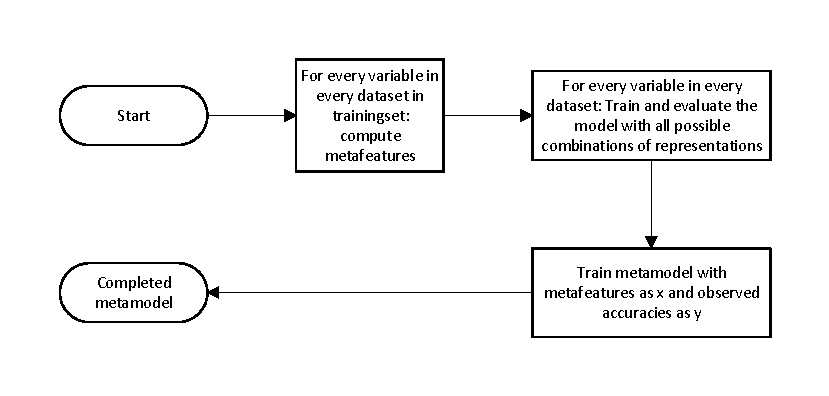
\includegraphics[width=.45\textwidth]{Drawing4.pdf}
\caption{Flowchart of the metamodel creation}
\label{fig_metamodel}
\end{figure}

\begin{figure}[!t]
\centering
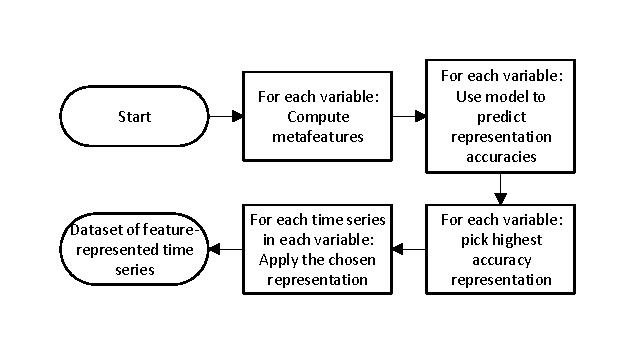
\includegraphics[width=.45\textwidth]{Drawing2.pdf}
\caption{Flowchart of the runtime usecase}
\label{fig_runtime}
\end{figure}

\begin{figure}
  \begin{algorithmic}[1] % for line numbering
    \REQUIRE Dataset consisting of (time, measure, label)
    \STATE $dataset \leftarrow pivot(dataset).groupBy(measure)$
    \FORALL{$(measure, TS, class) \in dataset$}
    \FORALL{$f \in Meta feature extractors$}
    \STATE $X_{(measure, f)} \leftarrow f(TS)$
    \ENDFOR
    \ENDFOR
  \end{algorithmic}
  \caption{Algorithm to generate features for the meta-model training-set}\label{gen-meta-xs}
\end{figure}

To generate the training-set we try to establish the accuracy of each possible representation as applied to the base classifier. This is done in a manner similar to forward construction of features. Thus the correct label becomes the feature configuration leading to the greatest increase in accuracy. The size of the training set can be chosen based on how accurate the user wants the feature-selection model needs to be. Algorithm \ref{gen-meta-ys} explains these steps in pseudo-code.

\begin{figure}
  \begin{algorithmic}[1] % for line numbering
    \REQUIRE $Dataset$, consisting of patient no., time, measure
    \REQUIRE $Y$, a vector of boolean values indicating the label
    \REQUIRE $TS$, a set of vectors of timeseries
    \REQUIRE $F = \left\{ f:vector \rightarrow \mathbb{R}\right\} $

    \FORALL{$t \in TS$}
    \FORALL{$e \in \mathcal{P}_{\geq 1}(F) $}
    \STATE $X_{f} \leftarrow f(t)$ \textbf{for all} $f \in e$
    \STATE $Y_{train}, Y_{test} \leftarrow SplitTrainingSet(Y)$
    \STATE $X_{train}, X_{test} \leftarrow SplitTrainingSet(X)$
    \STATE $BaseClf \leftarrow BuildBaseClassif(X_{train}, Y_{train})$
    \STATE $MetaY_{t, e} \leftarrow EvalClassif(BaseClf, Y_{train}, Y_{test})$
    \ENDFOR
    \ENDFOR
  \end{algorithmic}
  \caption{Algorithm to generate Y's for the meta-model training-set}\label{gen-meta-ys}
\end{figure}


After the training-set has been generated, all variables not included in the training-set are predicted using the feature-selection model, resulting in a set of features to be used for those time series (see figure \ref{fig_runtime}). 

This is done using a random forest algorithm which predicts the accuracy of the different representations. By outputting the accuracy for every possibility instead of just the label for the best representation, the differences between the performances of representation feature-sets can be seen. For example, it is possible to compare the best and the second-best representation. Thus, a cost function could be added and weigh improved accuracy against the cost of adding another necessary calculation for additional representations.

Finally, using the predicted as well as the train-set labels we apply those feature extraction function to each instance of each time-series variable, creating a feature vector for each individual in the data-set.

By applying the method outlined in this section, we believe that the accuracy can be improved or kept constant while dimensionality has been reduced. In the methodology section we will outline how this suggested technique was evaluated.

\subsection{Features}
The features used in the present study are the same as were used by Zhao et al., \cite{zhao2014}. This choice was made so as to isolate the effects of the technique itself rather than the available representations. The representations used in present studies are: 
\begin{enumerate}
    \item \emph{Existence:} 1, if the measurement exists for that patient, 0 otherwise
    \item \emph{Count:} The number of measurements in the time series, or 0 if the measurement was not done
    \item \emph{Mean:} The mean value of the measurements in the time series
    \item \emph{Stdev:} The standard deviation of that measurement per patient
    \item \emph{Slope:} ``The difference between the first and the last measurement value for each patient divided by the number of days in between''\cite{zhao2014}
\end{enumerate}

As we allow any combination of the above features, the number of possible representations (the number of combinations $N$) grows at at an exponential rate to the number of representation components, following the relationship $N = 2^n$ (see figure \ref{fig_powerset} for a visualization). Thus, for these five measurements, there are 31 representations excluding the empty set. All combinations need to be considered because additional representations can have an adverse or a beneficial effect on the accuracy of the classification.

\begin{figure}[!t]
\centering
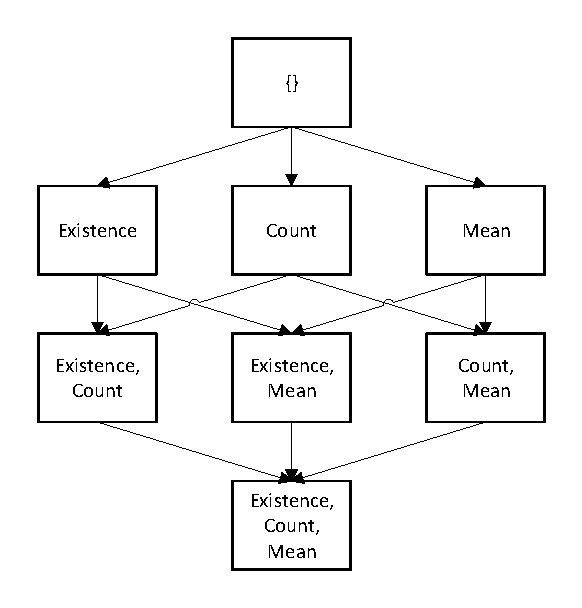
\includegraphics[width=.45\textwidth]{Drawing7.pdf}
\caption{Visualization of the lattice formed by the powerset of features (three out of five features included). These form all the possible representations.}
\label{fig_powerset}
\end{figure}

\subsection{Meta-features}
Meta-features are used by the random forest to decide on the best representation for a given time series. They are features describing whole columns, i.e., the measurement over all patients in the dataset, as opposed to the features which are calculated per patient. The meta-features are necessary in order to be able to compare different time series without domain knowledge, as domain knowledge would make the model not universally applicable. While the decision if a patient suffers from an ADE is obviously done per-patient, the representation of how their time series are represented need to consider the complete universe of time series of that measurement.

The following column meta-features are calculated to base the decision of the random forest on:
\begin{enumerate}
    \item \emph{Variance:} The variance of the measurement of all patients
    \item \emph{F-Test:} Total variance divided by the variance of the measurements within a patient 
    \item \emph{Mean:} Total mean of that column
    \item \emph{Median:} Total median of that column
    \item \emph{Average count per patient:} Averaged count of the measurement per patient
    \item \emph{Fraction of existence:} Fraction of patients who contain that measurement code
    
\end{enumerate}


\section{Methodology}


In order to answer the research question, we have chosen to use experimental methods. This choice was made because we wanted to collect several observations so as to be able to test the hypothesises inherent in our research question. Because the algorithm is new there was no other viable data-source other than creating it in the setting of an experiment. For this reason, experimental methods are the best option to structure this research.

In order to create the meta-model some data must be retained from the ADE dataset. There are 32 data files with a total of 3.62 million lines, each row consisting of the tuple (patient number, time of measurement, measurement code, measurement value, ADE class label). By grouping by measurement code and patient number and displaying the values over the time axis, timeseries are created. the ADE class label is used to calculate the accuracy of the prediction.

For the purpose of creating the meta-model a subset consisting of five out of the 32 data files were used. The remaining data files containing 3.29 million lines were treated as individual observations of the application of the technique, such that each individual data file is treated as independent of the others. 

This leaves a remaining 27 data-files for evaluation purposes. For each data-file, we then apply both the technique proposed in the present study and the approach of Zhao et al. \cite{zhao2014}. From this process the number of features generated by the naive approach, the number of features generated by the technique proposed in the present study as well as the accuracy of the naive and proposed approach were retained. This allows for making pair-wise comparisons of the accuracy of each model, thereby maximizing the statistical power of the hypothesis testing.

\subsection{Design of the experiment software}
For both the base model and the meta-model, random forests with 100 trees were constructed.
To calculate these random forests, Python 2.7.13 with Pandas \cite{mckinney-proc-scipy-2010}, Scipy \cite{scipy} and Scikit-learn \cite{scikit-learn} was used.
Initialization parameters for the random forest were $n_{estimators}=100$ and $max_{features}=\infty$, setting the number of trees to 100 and unsetting the number for the maximum features to guarantee that all features are considered for each branch, which is advantageous due to the sparsity of the dataset.

\subsection{Data analysis}
For statistical analysis the R environment was used\cite{rlang2016}. We computed descriptive statistics and Kernel Density Estimates (KDE) for the experimental data-set. Correlations between the number of features generated for each approach and the accuracy was computed using Spearman's rank-correlation coefficient, which is non-parametric. Using Spearman's rank-correlation coefficient is necessary because the measured accuracy of machine learning algorithms cannot be assumed to follow a Gaussian distribution forcing the use a non-parametric test, which to have lower power.

To compare the accuracy and number of features of the two methods we used the Wilcoxon signed-rank test for paired samples \cite{wilcoxon1945}. The Wilcoxon test is chosen for the same reasons as the Spearman's rank-correlation coefficient, as it is also non-parametric.

\section{Results}
The experimental data-set ($N=27$) showed mean accuracies of $31.59\%$ ($S=30.16$) for the naive approach and $31.96\%$ ($S=0.3133$) for the proposed approach, as can be seen in table \ref{resultstable}. Using the proposed approach resulted in reductions of accuracy in 10 cases, with the largest reduction being $8.571\%$. In 13 cases, the proposed technique outperformed the naive approach, with a maximum increase of $18.86\%$. The rank correlation of the accuracies $\rho$ was $0.9786$, which was significant ($t=23.779$, $df=25$, $p < 0.001$). A pair-wise Wilcoxon signed rank test revealed no significant difference for the accuracy of the two approaches ($V=139$, $p > 0.05$).

The average number of features using the naive approach was $1085$ ($S = 349.1$), whereas the average for the proposed approach was $630.5$ ($S = 204.5$). The average reduction of features was $455.3$ ($S = 148.5$) with a minimum reduction of 98 features and a maximum of 733. A KDE of the number of features generated is presented in figure \ref{fig_features_kde}. The proposed algorithm retained, on average $58.08\%$ ($S = 3.026$) of the full feature set. Indeed, a significant difference in the number of features was found between the two approaches ($V = 0$, $p < 0.001$).

\begin{figure}[!t]
\centering
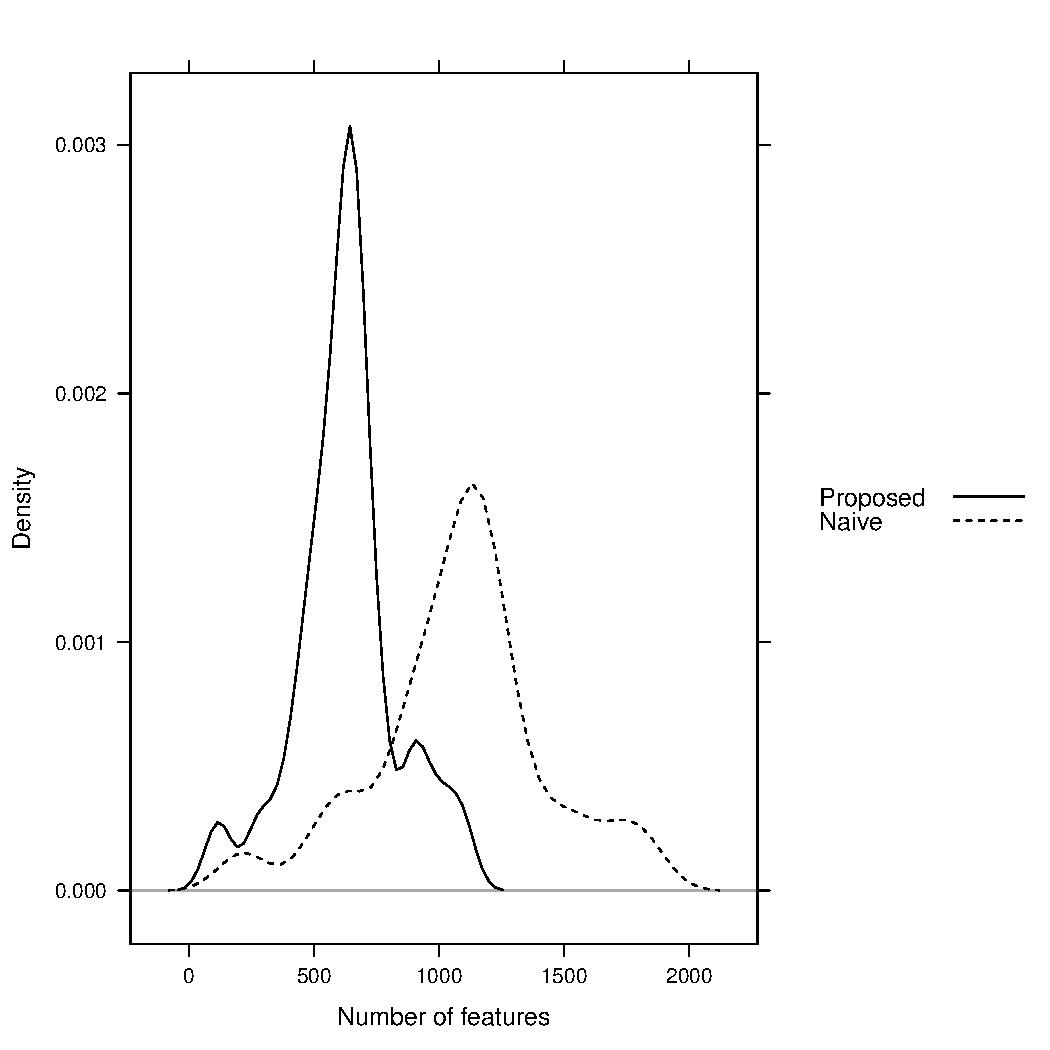
\includegraphics[width=.45\textwidth]{features_kde.pdf}
\caption{KDE for the number of features generated by each approach}
\label{fig_features_kde}
\end{figure}

\section{Discussion}

The main finding of the present study was a significant effect in the number of features, the proposed technique resulted in fewer features being generated. Additionally, no significant effect of accuracy was found, indicating that the technique performs on par with the naive approach, despite it using fewer features.

Our results indicate that the proposed technique is able to reduce the number of features while retaining similar accuracy to the full representation. This demonstrates the effectiveness of the technique proposed in this study for choosing the optimal representations of time-series. We believe that this approach, if developed further, could be appropriate for both research and industry use. Before recommending such use, however, future research is required.

The present study only applied the developed technique only to a single kind of data-set, the data-sets are all data concerning the existence of ADEs and the features are all extremely sparse time-series. Future research could apply the technique proposed in this paper to other datasets. Another avenue for future research can be found in modifying the technique to use different features and meta-features. Finally, because the proposed approach doesn't require that random forests are used, other regression models such as artificial neural networks and support vector machines could be used.

There is room for improvement in the construction of the meta-model in the current implementation complete random forests are rebuilt for every possible feature set. A more efficient approach would be to build a single random forest without the feature presently considered, and then additional decision trees using a stratified sample of the features presently considered. This optimization can be taken further by initially building a random forest using the maximal representation of each feature and then pruning it of trees containing the feature under consideration. This would improve the performance of the algorithm significantly.


Also, other approaches could be taken into consideration to account for unbalanced class labels in the datasets. These are to be expected as only a small part of diseases are likely to be caused by ADEs.

Despite the limitations and need for future research the approach shows promise, and with the proposed adjustments, could present an improvement of the state of the art in this particular niche.


\begin{table}[!t]
\centering
\caption{Results of the random forest meta-model}
\label{resultstable}
\begin{tabular}{l|lllll}
Dataset & $feat_{naive}$ & $feat_{smart}$ & $acc_{naive}$ & $acc_{smart}$ & $Delta$   \\ \hline
1  & 1083           & 603            & 0.2914        & 0.3429        & 0.05143   \\
2  & 1824           & 1091           & 0.8484        & 0.8225        & -0.02588  \\
3  & 1563           & 892            & 0.1072        & 0.119         & 0.01178   \\
4  & 1017           & 575            & 0.8565        & 0.8333        & -0.02315  \\
5  & 966            & 576            & 0.3214        & 0.2589        & -0.0625   \\
6  & 1014           & 618            & 0.01205       & 0.01205       & 0         \\
7  & 642            & 449            & 0.1714        & 0.08571       & -0.08571  \\
8  & 846            & 476            & 0.4717        & 0.6604        & 0.1887    \\
9  & 1116           & 641            & 0.5761        & 0.5246        & -0.05152  \\
10 & 981            & 551            & 0.35          & 0.3364        & -0.01364  \\
11 & 1089           & 634            & 0.6368        & 0.6547        & 0.01794   \\
12 & 1224           & 689            & 0.1168        & 0.07977       & -0.03704  \\
13 & 1155           & 677            & 0.006135      & 0             & -0.006135 \\
14 & 1155           & 683            & 0.07362       & 0.04908       & -0.02454  \\
15 & 1476           & 913            & 0.7409        & 0.7929        & 0.05198   \\
16 & 510            & 282            & 0             & 0             & 0         \\
17 & 639            & 387            & 0.04902       & 0.04902       & 0         \\
18 & 1722           & 1004           & 0.6992        & 0.7182        & 0.01903   \\
19 & 216            & 118            & 0             & 0             & 0         \\
20 & 1179           & 654            & 0.1008        & 0.129         & 0.02823   \\
21 & 1179           & 659            & 0.01984       & 0.02381       & 0.003968  \\
22 & 1179           & 659            & 0.004032      & 0.0121        & 0.008065  \\
23 & 1179           & 658            & 0.8252        & 0.8659        & 0.04065   \\
24 & 870            & 510            & 0.3314        & 0.3373        & 0.005917  \\
25 & 867            & 509            & 0.5385        & 0.568         & 0.02959   \\
26 & 1314           & 763            & 0.3835        & 0.3509        & -0.03258  \\
27 & 1314           & 754            & 0             & 0.005         & 0.005    
\end{tabular}
\end{table}



% needed in second column of first page if using \IEEEpubid
%\IEEEpubidadjcol

% An example of a floating figure using the graphicx package.
% Note that \label must occur AFTER (or within) \caption.
% For figures, \caption should occur after the \includegraphics.
% Note that IEEEtran v1.7 and later has special internal code that
% is designed to preserve the operation of \label within \caption
% even when the captionsoff option is in effect. However, because
% of issues like this, it may be the safest practice to put all your
% \label just after \caption rather than within \caption{}.
%
% Reminder: the "draftcls" or "draftclsnofoot", not "draft", class
% option should be used if it is desired that the figures are to be
% displayed while in draft mode.
%
%\begin{figure}[!t]
%\centering
%\includegraphics[width=2.5in]{myfigure}
% where an .eps filename suffix will be assumed under latex,
% and a .pdf suffix will be assumed for pdflatex; or what has been declared
% via \DeclareGraphicsExtensions.
%\caption{Simulation Results}
%\label{fig_sim}
%\end{figure}

% Note that IEEE typically puts floats only at the top, even when this
% results in a large percentage of a column being occupied by floats.


% An example of a double column floating figure using two subfigures.
% (The subfig.sty package must be loaded for this to work.)
% The subfigure \label commands are set within each subfloat command, the
% \label for the overall figure must come after \caption.
% \hfil must be used as a separator to get equal spacing.
% The subfigure.sty package works much the same way, except \subfigure is
% used instead of \subfloat.
%
%\begin{figure*}[!t]
%\centerline{\subfloat[Case I]\includegraphics[width=2.5in]{subfigcase1}%
%\label{fig_first_case}}
%\hfil
%\subfloat[Case II]{\includegraphics[width=2.5in]{subfigcase2}%
%\label{fig_second_case}}}
%\caption{Simulation results}
%\label{fig_sim}
%\end{figure*}
%
% Note that often IEEE papers with subfigures do not employ subfigure
% captions (using the optional argument to \subfloat), but instead will
% reference/describe all of them (a), (b), etc., within the main caption.


% An example of a floating table. Note that, for IEEE style tables, the
% \caption command should come BEFORE the table. Table text will default to
% \footnotesize as IEEE normally uses this smaller font for tables.
% The \label must come after \caption as always.
%
%\begin{table}[!t]
%% increase table row spacing, adjust to taste
%\renewcommand{\arraystretch}{1.3}
% if using array.sty, it might be a good idea to tweak the value of
% \extrarowheight as needed to properly center the text within the cells
%\caption{An Example of a Table}
%\label{table_example}
%\centering
%% Some packages, such as MDW tools, offer better commands for making tables
%% than the plain LaTeX2e tabular which is used here.
%\begin{tabular}{|c||c|}
%\hline
%One & Two\\
%\hline
%Three & Four\\
%\hline
%\end{tabular}
%\end{table}


% Note that IEEE does not put floats in the very first column - or typically
% anywhere on the first page for that matter. Also, in-text middle ("here")
% positioning is not used. Most IEEE journals use top floats exclusively.
% Note that, LaTeX2e, unlike IEEE journals, places footnotes above bottom
% floats. This can be corrected via the \fnbelowfloat command of the
% stfloats package.




% if have a single appendix:
%\appendix[Proof of the Zonklar Equations]
% or
%\appendix  % for no appendix heading
% do not use \section anymore after \appendix, only \section*
% is possibly needed

% use appendices with more than one appendix
% then use \section to start each appendix
% you must declare a \section before using any
% \subsection or using \label (\appendices by itself
% starts a section numbered zero.)
%


%\appendices
%\section{Proof of the First Zonklar Equation}
%\blindtext

% use section* for acknowledgement
%\section*{Acknowledgment}


%The authors would like to thank...


% Can use something like this to put references on a page
% by themselves when using endfloat and the captionsoff option.
\ifCLASSOPTIONcaptionsoff
  \newpage
\fi



% trigger a \newpage just before the given reference
% number - used to balance the columns on the last page
% adjust value as needed - may need to be readjusted if
% the document is modified later
%\IEEEtriggeratref{8}
% The "triggered" command can be changed if desired:
%\IEEEtriggercmd{\enlargethispage{-5in}}

% references section

% can use a bibliography generated by BibTeX as a .bbl file
% BibTeX documentation can be easily obtained at:
% http://www.ctan.org/tex-archive/biblio/bibtex/contrib/doc/
% The IEEEtran BibTeX style support page is at:
% http://www.michaelshell.org/tex/ieeetran/bibtex/
\bibliographystyle{IEEEtran}
% argument is your BibTeX string definitions and bibliography database(s)
\bibliography{IEEEabrv,bibliography}
%
% <OR> manually copy in the resultant .bbl file
% set second argument of \begin to the number of references
% (used to reserve space for the reference number labels box)
%\begin{thebibliography}{1}

%\bibitem{IEEEhowto:kopka}
%H.~Kopka and P.~W. Daly, \emph{A Guide to \LaTeX}, %3rd~ed.\hskip 1em plus
%  0.5em minus 0.4em\relax Harlow, England: Addison-Wesley, 1999.

%\end{thebibliography}

% biography section
%
% If you have an EPS/PDF photo (graphicx package needed) extra braces are
% needed around the contents of the optional argument to biography to prevent
% the LaTeX parser from getting confused when it sees the complicated
% \includegraphics command within an optional argument. (You could create
% your own custom macro containing the \includegraphics command to make things
% simpler here.)
%\begin{biography}[{\includegraphics[width=1in,height=1.25in,clip,keepaspectratio]{mshell}}]{Michael Shell}
% or if you just want to reserve a space for a photo:

\begin{IEEEbiography}[{\includegraphics[width=1in,height=1.25in,clip,keepaspectratio]{picture}}]{John Doe}
\blindtext
\end{IEEEbiography}

% You can push biographies down or up by placing
% a \vfill before or after them. The appropriate
% use of \vfill depends on what kind of text is
% on the last page and whether or not the columns
% are being equalized.

%\vfill

% Can be used to pull up biographies so that the bottom of the last one
% is flush with the other column.
%\enlargethispage{-5in}




% that's all folks
\end{document}
